\documentclass[11pt, a4paper]{article}
\usepackage[margin=0.95in]{geometry}
\usepackage{amsmath}
\usepackage{amsfonts}
\usepackage{graphicx}
\usepackage{tikz}
\graphicspath{ {./} }
\usepackage{mathtools}
\DeclarePairedDelimiter{\abs}{\lvert}{\rvert}
\usetikzlibrary{automata,positioning} % automata and positioning libraries are required to use nodes and coordinates in addition to placement propetries.
%\usepackage{parskip}
% equations coulde be %   default number of the equation on the rigth and equation centered 
%   leqno number on the left and equation centered %   fleqn number on the rigth and  equation on the left side
\newcommand{\solution}{ \noindent \textbf{Solution:}}
\newcommand{\problem}[1]{\textit{#1} \medskip}

% get rid of spacing after problem headers
\usepackage{titlesec}
%\titlespacing\subsection{0pt}{12pt plus 4pt minus 2pt}{0pt plus 2pt minus 2pt}
\titlespacing{\subsection}{0pt}{*3}{-\parskip}

\newcommand{\icol}[1]{% inline column vector
  \left(\begin{smallmatrix}#1\end{smallmatrix}\right)%
}

\newcommand{\irow}[1]{% inline row vector
  \begin{smallmatrix}(#1)\end{smallmatrix}%
}

\title{Combinatorial Optimization and Modern Heuristics: Assignment 1}
\author{
	Max Williams\\
    \textsc{Computer Science \& Engineering}\\
	\and 
    Luke Floden [\textsc{contributor}]\\
    \textsc{Computer Science \& Engineering}\\
	}

\date{\today} 
\begin{document}
\maketitle


\section*{Chapter 1 Problems}

\subsection*{Problem 1(d)}

\problem{Find a cylinder with a given surface area A that has the largest volume $V$.}

\solution

For the solution, it is sufficient to give only a feasible set $F$ and cost function $c$.

\begin{align}
    F &= \{r,h\in \mathbb{R}: 2\pi r(h+r)=A\}\\
    c &= \frac{1}{\pi r^2 h}, c:F\to \mathbb{R}
\end{align}


\subsection*{Problem 3}

\problem{Show that the neighborhood defined in Example 1.5 for the MST is exact.}

\includegraphics[scale=0.4]{ex15}

\solution

\newcommand{\len}{\text{len}}

Assume there is a spanning tree $L$ which is locally optimal but not globally optimal. Also take the
globally optimal spanning tree $G$ which \emph{has the most edges in common with $L$}. We pick an
edge $e_1$ from $G$ which is not in $L$ and divide the vertices into sets $G_1$ and $G_2$. 
We define the set $Q$ to be the set of edges in $L$ such that each edge in $Q$ both has one vertice
in $G_1$ and one vertice in $G_2$ and belongs to the cycle created when $e_1$ is added to $L$. We
select $e_2$ as an arbitrary edge in $Q$.

From the assumption that $L$ is locally optimal,
we know that replacing $e_1$ with $e_2$ in $L$ would lead to an increase in (or no change to) the
cost of $L$, thus $\len(e_1) \geq \len(e_2)$. However, the assumption that $G$ is globally opimal
similarly implies that $\len(e_1) \leq \len(e_2)$. Thus we know that $\len(e_1) = \len(e_2)$. 

Since $e_1$ and $e_2$ have the same length, then $e_1$ in $G$ could be replaced with $e_2$ to give
the spanning tree $G'$ which is also a globally minimal spanning tree. This contradicts the
assumption that $G$ is a globally minimal spanning tree which shares the most edges with $L$, as we
have found globally optimal $G'$ which shares one additional edge with $L$. Thus we conclude that
our assumption that $L$ could be locally optimal but not globally optimal was incorrect.



\begin{figure}[!h]
\centering
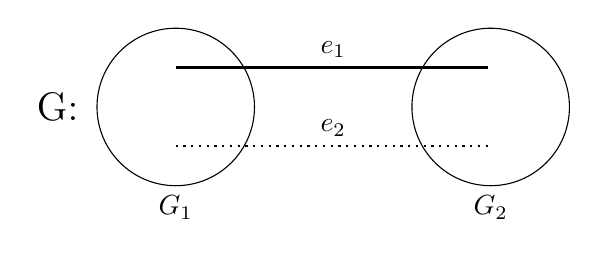
\begin{tikzpicture}[shorten >=1pt,node distance=1.0cm,on grid,auto]
    \node[state,circle, align=center,minimum size=2cm] at (0,0) (q1) [label=below:$G_1$] {};
    \node[state,circle, align=center,minimum size=2cm]  at (4,0) (q2) [label=below:$G_2$] {};
    \path[thick] (0,.5) edge  node  {$e_1$} (4,.5);
    \path[dotted, thick] (0,-.5) edge  node  {$e_2$} (4,-.5);
    \node[] at (-1.5,0) {\Large G:};
\end{tikzpicture}
    \caption{Globally optimal tree $G$ with edge $e_1$ in the tree and $e_2$ not in the tree.}
    \label{fig:g}

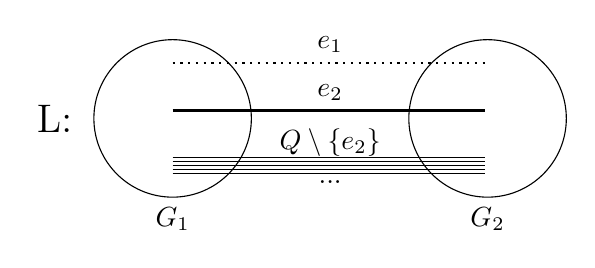
\begin{tikzpicture}[shorten >=1pt,node distance=1.0cm,on grid,auto]
    \node[state,circle, align=center,minimum size=2cm] at (0,0) (q1) [label=below:$G_1$] {};
    \node[state,circle, align=center,minimum size=2cm]  at (4,0) (q2) [label=below:$G_2$] {};
    \path[dotted, thick] (0,.7) edge  node  {$e_1$} (4,.7);
    \path[thick] (0,.1) edge  node  {$e_2$} (4,.1);

    \path[] (0,-.5) edge  node[yshift=-3]  {$Q\setminus \{e_2\}$} (4,-.5);
    \foreach \dy in {-.55, -.6, -.65}
        \path[] (0,\dy) edge  (4,\dy);
    \path[] (0,-.7) edge  node[below, yshift=1] {...}(4,-.7);
    \node[] at (-1.5,0) {\Large L:};
\end{tikzpicture}
    \caption{Locally optimal tree $L$ with edge $e_2$ in the tree that would form a cycle is $e_1$
    were added to the tree.  Set of superfluous edges $Q$ is also shown.}
    \label{fig:l}
\end{figure}

\subsection*{Problem 6}

\problem{Suppose we are given a set $S$ containing $2n$ integers, and we wish to partition it into
two sets $S_1$ and $S_2$ so that $\abs{S_1}=\abs{S_2}=n$ and so that the sum of the numbers in $S_1$
is as close as possible to the sum of those in $S_2$. Let the neighborhood $N$ be determined by all
possible interchanges of two integers between $S_1$ and $S_2$. Is $N$ exact?}

\solution


The given neighborhood is not exact. There exists two sets such that, in this neighborhood, they are
locally optimal but they are not the global optimum. The sets are $S_1 = \{1, 2, 8, 9\}$ and $S_2 =
\{3, 4, 5, 6\}$. Their sums are 20 and 18, respectively. By exchanging any two elements, the
difference in their sums cannot be decreased. However, the sets $\{1, 3, 6, 9\}$ and 
$\{2, 4, 5, 8\}$ sum to 19 and 19 respectively: a difference of 0. Thus the neighborhood is not
exact.


\subsection*{Problem 9}
\newcommand{\convexity}[1]{
\begin{equation}
    #1(\la\x+(1-\la)\y) \leq \la #1(\x)+(1-\la) #1(\y), \la \in \mathbb{R}\ \text{and}\ 0\leq\la\leq1
\end{equation}
}

\problem{Let $f(x)$ be convex in $R^n$. Fix $x_2,...,x_n$ and consider the function $g(x_1) =
f(x_1,...,x_n)$. Is $g$ convex in $R^1$?}

\solution

Using the definition of convexity, we have

\newcommand{\la}{\lambda}
\newcommand{\x}{\bar{x}}
\newcommand{\y}{\bar{y}}
\convexity{f}


We can rewrite $\x$ and $\y$ as vectors 
\newcommand{\vecrange}[2]{\langle #1, ...\ , #2 \rangle}
\renewcommand{\x}{\vecrange{x_1}{x_n}}
\renewcommand{\y}{\vecrange{y_1}{y_n}}
$\x$ and $\y$.

\begin{equation}
    f(\la\x+(1-\la)\y) \leq \la f(\x)+(1-\la) f(\y), \la \in \mathbb{R}
\end{equation}

Then do some linear algebra to arrange this so that the substitution for $g(x_1)$ becomes possible

\begin{align}
    f(\vecrange{\la x_1+(1-\la) y_1}{\la x_n+(1-\la) y_n}) &\leq \la f(\x)+(1-\la) f(\y)\\
    g(\la x_1+(1-\la) y_1) &\leq \la g(x_1)+(1-\la) g(x_1)
\end{align}

Which is precisely the statement that $g(x_1)$ is convex in $\mathbb{R}^1$.


\subsection*{Problem 10}

\problem{Let $f(x_i)$ be a convex function of the single variable $x_i$. Then $g(x) = f(x_i)$ can also
be considered a function of $x \in R^n$. Is $g(x)$ convex in $R^n$?}

\solution

Since $g$ ignores all of the elements of $\bar{x}$, then it is constant along all dimensions except
for the $i$th dimension. Thus $g(\bar{x})$ is convex. To prove this formally, first we state $f$'s
convexity formally.

\renewcommand{\x}{x_i}
\renewcommand{\y}{y_i}
\convexity{f}

The right hand side can be substituted with $g$, creating vectors $\bar{x}$ and $\bar{y}$ which have
$x_i$ and $y_i$ as their $i$th elements, respectively. The left hand side is more complicated.
When the substitution is performed, a vector with $\la \x+(1-\la)\y$ as the $i$th element is made,
with the remaining elements arbitrary. This vector is equal to $\la \bar{x} + (1-\la)\bar{y}$ at
index $i$, and the remaining values in the vector are ignored. Thus we can finally state

\renewcommand{\x}{\bar{x}}
\renewcommand{\y}{\bar{y}}
\convexity{g}

\section*{Chapter 2 Problems}

\subsection*{Problem 8}

\problem{Show that the set of optimal points of an instance of LP is a convex set.}

\solution

The set of feasible solutions $C: \mathbb{R}^n$ for an LP are defined as
\begin{equation}
    C=\{\bar{x}\in\mathbb{R}^n | \boldsymbol{A}\bar{x} \geq \bar{b}\}. 
\end{equation}

With a linear cost function, $c: \mathbb{R}^n\to\mathbb{R}$,  we can
define the set of optimal points, $S$, as
\begin{equation}
    S=\{\bar{x}\in\mathbb{R}^n | \boldsymbol{A}\bar{x} \geq \bar{b}\ \text{and}\ c(\bar{x})=v\} 
\end{equation}

where $v$ is the value such that $\forall x\in C: c(x) \leq v$.

Using the definition of a convex set:
\begin{equation}
    \forall \bar{y_1}, \bar{y_2} \in C: \la \bar{y_1} + (1-\la) \bar{y_2} \in C, 0 \leq \la \leq 1
\end{equation}

First we show that the set of feasible solutions is convex. Given $\bar{y_1}, \bar{y_2} \in C$, we show that
their convex combination is also in $C$. 

\begin{align}
    \la\boldsymbol{A}(\bar{y_1}) &\geq \la b\\
    (1-\la)\boldsymbol{A}(\bar{y_2}) &\geq (1-\la)b\\
    \boldsymbol{A}(\la \bar{y_1} + (1-\la) \bar{y_2}) &=  \la\boldsymbol{A}(\bar{y_1}) +
    (1-\la)\boldsymbol{A}(\bar{y_2}) \\
    \la\boldsymbol{A}(\bar{y_1}) + (1-\la)\boldsymbol{A}(\bar{y_2}) &\geq \la b + (1-\la)b = b
\end{align}

Next we need to show that the set of optimal points is convex. Given $\bar{y_1}, \bar{y_2} \in S$, we want to
show that $\la \bar{y_1} + (1-\la) \bar{y_2} \in C.$ Since we already know that $C$ is a convex set, we only
need to take care of the optimality constraint. Given $c(\bar{y_1}) = v, c(\bar{y_2}) = v$, we need to show that
their convex combination also equals $v$. This is fairly easy thanks to $c$'s linearity.

\begin{equation}
    c(\la \bar{y_1} + (1-\la) \bar{y_2}) = \la c(\bar{y_1}) + (1-\la) c(\bar{y_2}) = \la v + (1-\la)v = v
\end{equation}

Taken together, this means the set of optimal points (that is, points that are both feasible and
have a cost equal to $v$) is convex.

\end{document}
